\newpage
\section{Auswertung}
\subsection{Abhängigkeit der Ausgangsspannung von der Phasenverschiebung}
In den folgenden Abbildungen werden die Spannungsverläufe für einzelne Phasen aufgezeigt.
Hierbei werden Phasenunterschiede von $\varphi = 90^\circ, 135^\circ, 180^\circ, 225^\circ$und $270^\circ$ dargestellt. 

\begin{figure}[H]
    \begin{minipage}{0.4\textwidth}
     \centering
      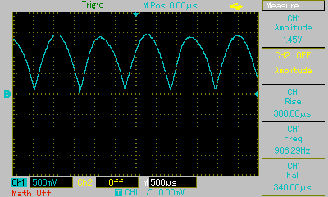
\includegraphics[width=0.8\textwidth]{Auswertung/1.pdf}
      \caption{$\varphi = 90^\circ$}
	\label{fig:uno}
    \end{minipage}\hfill
    \begin{minipage}{0.4\textwidth}
     \centering
      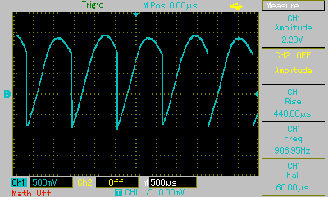
\includegraphics[width=0.8\textwidth]{Auswertung/2.pdf}
      \caption{$\varphi = 135^\circ$}
	\label{fig:dos}
    \end{minipage}
\end{figure}

\begin{figure}[h]
    \begin{minipage}{0.4\textwidth}
     \centering
      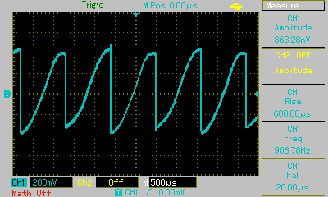
\includegraphics[width=0.8\textwidth]{Auswertung/3.pdf}
      \caption{$\varphi = 180^\circ$}
	\label{fig:tres}
    \end{minipage}\hfill
    \begin{minipage}{0.4\textwidth}
     \centering
      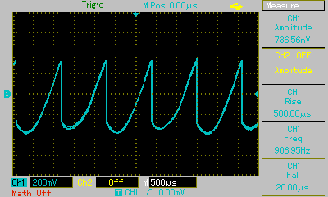
\includegraphics[width=0.8\textwidth]{Auswertung/4.pdf}
      \caption{$\varphi = 225^\circ$}
	\label{fig:qua}
    \end{minipage}
\end{figure}

\begin{figure}[h]
    \centering
    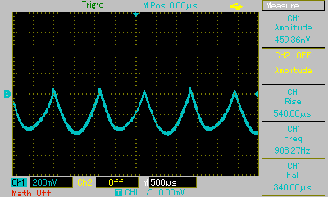
\includegraphics[width=0.32\textwidth]{Auswertung/5.pdf}
    \caption{$\varphi = 270^\circ$}
	\label{fig:sinco}
\end{figure}

In der folgenden Tabelle sind die gemessenen Amplituden bei verschiedenen Phasendifferenzen, einmal mit und einmal ohne Störsignal (Rauschen), aufgezeigt.
\begin{table}
\begin{minipage}{0.5\textwidth}
	\centering
	\caption{Phasenunterschied ohne Rauschen.}
	\label{tab:a}
	\begin{tabular}{c|c}
		\toprule
		{$\varphi / \circ $} & {$U_\text{A} / \text{V}$} \\
		\hline
		\midrule
		0 & -3,8 \\
		15 & -4,4 \\
		30 & -5,6 \\
		45 & -6,2 \\
		60 & -6,2 \\
		75 & -5,6 \\
		90 & -4,8 \\
		105 & -3,6 \\
		120 & -2,6 \\
		135 & -0,6 \\
		150 & 2,0 \\
		165 & 3,8 \\
		180 & 5,0 \\
		195 & 6,0 \\
		210 & 6,8 \\
		225 & 7,6 \\
		240 & 7,6 \\
		255 & 7,0 \\
		270 & 6,2 \\
		285 & 5,2 \\
		300 & 4,0 \\
		315 & 1,8 \\
		330 & -0,6 \\
		345 & -2,4 \\
		360 & -3,8 \\
		\bottomrule 
	\end{tabular}
\end{minipage}
\begin{minipage}{0.5\textwidth}
	\centering
	\caption{Phasenabhängigkeit mit Rauschen.}
	\label{tab:b}
	\begin{tabular}{c|c}
		\toprule
		{$\varphi / \circ $} & {$U_\text{A} / \text{mV}$} \\
		\hline
		\midrule
		0 & -108 \\
		15 & -136 \\
		30 & -190\\
		45 & -198\\
		60 & -178\\
		75 & -168 \\
		90 & -138\\
		105 & -106 \\
		120 & -54\\
		135 & 34 \\
		150 & 82 \\
		165 & 122 \\
		180 & 140\\
		195 & 150\\
		210 & 180\\
		225 & 198\\
		240 & 224 \\
		255 & 216\\
		270 & 200\\
		285 & 180\\
		300 & 140\\
		315 & 80\\
		330 & 0 \\
		345 & -64 \\
		360 & -96 \\
		\bottomrule 
	\end{tabular}
\end{minipage}
\end{table}
\\
\\
Aus der Tabelle \ref{tab:a} ergibt sich der Graph \ref{fig:sinus}.
\begin{figure}[h]
	\centering
	\includegraphics{Sinus.pdf}
	\caption{Phasenabhängigkeit der Amplitude ohne Störsignal}
	\label{fig:sinus}
\end{figure}

Diese Funktion hat die Grundform
\begin{equation}
	y = A\cdot sin(B \cdot x + C) + D
\end{equation}
Dabei ist $y$ gegeben durch die Amplitude $U_A$ und $x$ durch die Phasenverschiebung $\varphi$. \\
Mittels Regression ergeben sich folgende Werte für die Parameter.
\begin{equation}
	A = \SI{-6.996 \pm 0.009}{V} \notag
\end{equation}
\begin{equation}
	B = \SI{1.11760 \pm 0.00007}{1/m} \notag
\end{equation}
\begin{equation}
	C = 0.6287 \pm 0.0009 \notag
\end{equation}
\begin{equation}
	D = \SI{0.704 \pm 0.005}{V} \notag
\end{equation}

Daraus lässt sich nun nach (5) und dem Parameter $A$, der die resultierende Gleichspannung $U_\text{out}$ darstellt, die Eingangsspannung $U_0$ bestimmen.
\begin{equation}
	U_0 = \frac{\pi}{2}U_\text{out}
\end{equation}
Somit ergibt sich $U_0 = \SI{10,99}{V}$.

Aus der Tabelle \ref{tab:b} ergibt sich folgender Graph für die Phasenabhängigkeit mit Störsignal.
\begin{figure}[h]
	\centering
	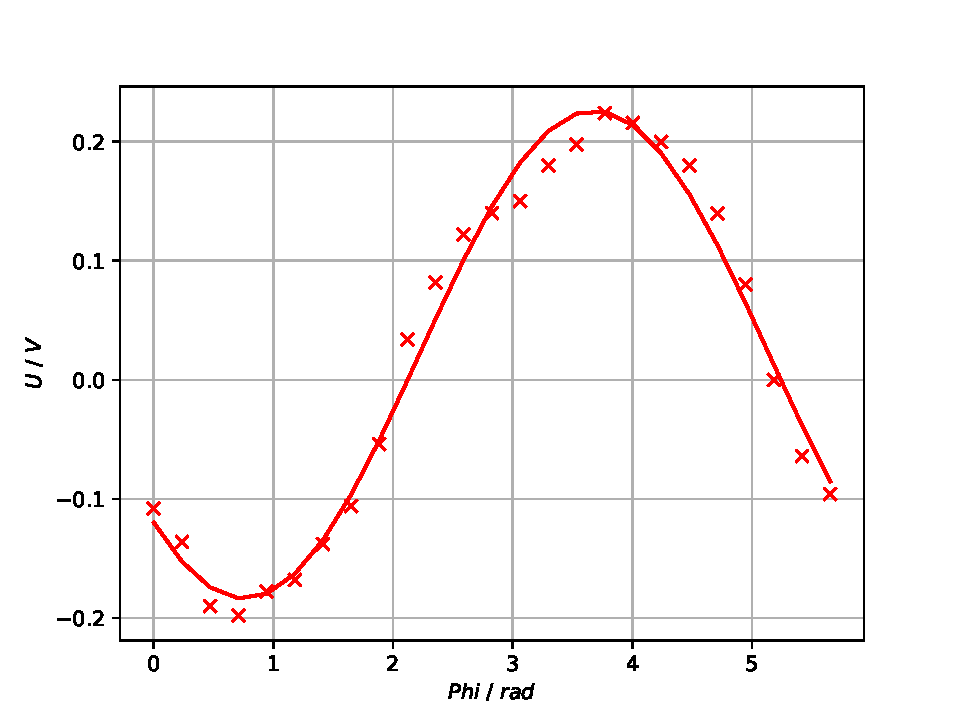
\includegraphics{Sinus2.pdf}
	\caption{Phasenabhängigkeit der Amplitude mit Störsignal}
	\label{fig:sinus2}
\end{figure}

Diese Ausgleichsfunktion hat ebenfalls die Form (6) und es ergeben sich durch Regression andere Paramter.
\begin{equation}
	A = \SI{-0.20500 \pm 0.00003}{V}\notag
\end{equation}
\begin{equation}
	B = \SI{1.0736 \pm 0.0004}{1/m} \notag
\end{equation}
\begin{equation}
	C = 0.759 \pm 0.005 \notag
\end{equation}
\begin{equation}
	D = \SI{0.02120 \pm 0.00002}{V} \notag
\end{equation}

Aus (5) und (7) lässt sich nun die Eingangsspannung auf $U_0 = \SI{0,31}{V}$ bestimmen.

\subsection{Rauschunterdrückung mit einer Photodetektorschaltung}
In der Tabelle \ref{tab:c} werden die Messwerte des Abstandes vom Detektor zur LED und der dazugehörigen gemessenen Spannung am Detektor, die die Intensiät widerspiegelt, aufgetragen.

\begin{table} [H]
	\centering
	\caption{Abhängigkeit der Intensität vom Abstand r.}
	\label{tab:c}
	\sisetup{table-format=3.2}
	\begin{tabular}{S[table-format=3.2] S S S S [table-format=3.2]}
		\toprule
		{$\text{Abstand} \; r / \text{cm}$} & {$U / \text{V} $} \\
		\midrule
		6 & 5,8 \\
		7 & 5,8 \\
		8 & 5,8 \\
		9 & 5,6 \\
		10 & 5,6 \\
		11 & 5,6 \\
		12 & 5,6 \\
		13 & 5,4 \\
		14 & 5,4 \\
		15 & 5,6 \\
		17 & 5,8 \\
		19 & 5,8 \\
		21 & 5,6 \\
		23 & 4,8 \\
		25 & 4,2 \\
		27 & 3,6 \\
		29 & 3,2 \\
		31 & 2,8 \\
		33 & 2,6 \\
		35 & 2,4 \\
		37 & 2,2 \\
		40 & 2,0 \\
		45 & 1,6 \\
		50 & 1,6 \\
		55 & 1,4 \\
		60 & 1,2 \\
		65 & 1,2 \\
		70 & 1,0 \\
		80 & 1,0 \\
		90 & 1,0 \\
		100 & 1,0\\
		\bottomrule 
	\end{tabular}
\end{table}

Allgemein folgt für die Funktion
\begin{equation}
	y = A \frac{1}{r^2} + B
\end{equation}
Dabei ist $y$ die Intensität bzw. die gemessene Spannung und $r$ der Abstand zwischen der LED und des Detektors.
Durch Regression ergeben sich folgende Parameter.
\begin{equation}
	A = \SI{1750.53 \pm 8503.20}{V \cdot m^2} \notag
\end{equation}
\begin{equation}
	B = \SI{0.916 \pm 0.016}{V} \notag
\end{equation}

Damit ergibt sich der folgende Graph.

\begin{figure}[h]
	\centering
	\includegraphics{led.pdf}
	\caption{Intensität in Abhängigkeit vom Abstand zur LED}
	\label{fig:led}
\end{figure}

Der maximale Abstand $r_\text{max}$ konnte experimentell nicht bestimmt werden, da die Möglichkeiten der Messapparaturen nicht ausreichend waren.
Es ergibt sich mit der Regression und der Annahme, dass die Steigung bei größer werdendem Abstand nahezu konstant ist der Wert
\begin{align}
	r_\text{max} = \SI{182,5}{cm}
\end{align}.
